\subsection{Parallélisation des méthodes itératives}
La partie résolution de système linéaire creux représente souvent la partie qui consomme le plus de temps dans une simulation numérique, par exemple dans la simulation de réservoir cela peut représenter jusqu'à 80~\% du temps de simulation.
%
Il est donc essentiel de paralléliser cette partie du code.
%
Les noyaux de calcul les plus coûteux du GMRES préconditionné sont :
\begin{itemize}
  \item la factorisation ILU;
  \item les résolutions triangulaires;
  \item le produit matrice vecteur creux;
  \item les produits scalaires.
\end{itemize}

La méthode parallélisation la plus répandue du GMRES est la méthode de Jacobi par blocs.
%
Dans cette méthode, nous découpons des blocs dans la matrice et nous appliquons une factorisation ILU par bloc.
%
Ces blocs proviennent d'un partitionnement du graphe d'adjacence de la matrice à l'aide d'un logiciel de partitionnement, tel que Scotch ou Metis, avec pour objectif un bon équilibrage de charge.

%   (-_-)   %
\begin{figure}[!h]
  \centering
  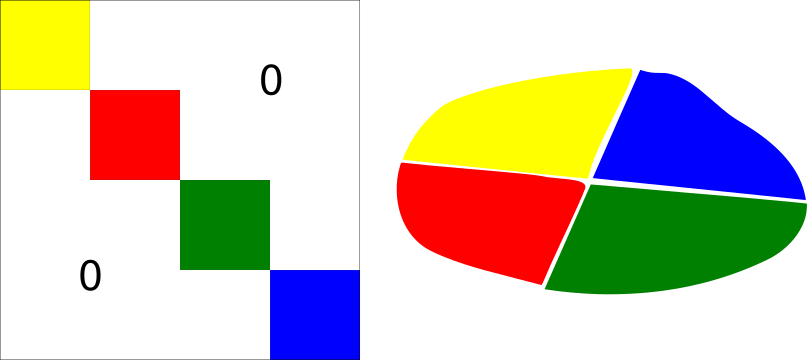
\includegraphics[width=\textwidth]{jacobi}
  \caption{Exemple de partitionnement.}
  \label{fig:jacobi}
\end{figure}
